%----------------------------------------------------------------------------------------
%	Hasil dan Pembahasan
%----------------------------------------------------------------------------------------
\section*{HASIL DAN PEMBAHASAN}

Penelitian yang dilakukan terbagi menjadi beberapa tahapan proses. 

\subsection*{Analisis}

Pada tahap ini dimulai dari membaca literatur terkait dan mengumpulkan beberapa contoh program yang akan digunakan dalam penelitian. Contoh program yang digunakan dalam penelitian ini didapatkan dari penelitian yang dilakukan oleh \citeauthor{HERMADI2015} (\cite*{HERMADI2015}).  

\textit{Basis path testing} merupakan salah satu metode pengujian struktural yang menggunakan \textit{source code} dari program untuk menemukan semua jalur yang mungkin dapat dilalui program dan dapat digunakan untuk merancang data uji. Metode ini memastikan semua kemungkinan jalur dijalankan setidaknya satu kali (\cite{BASU2015}). Metode ini terbagi menjadi 4 tahapan, yaitu:
\begin{enumerate}[noitemsep] 
	\item Menggambarkan jalur dalam bentuk \textit{ Control Flow Graph} (CFG)
	\item Menghitung \textit{cyclomatic complexity}
	\item Memilih satu set jalur dasar
	\item Membangkitkan data uji untuk setiap jalur dasar
\end{enumerate}

\textit{Control Flow Graph }(CFG) adalah graph berarah yang merepresentasikan aliran dari sebuah program. Setiap CFG terdiri dari \textit{nodes} dan \textit{edges}. \textit{Nodes} merepresentasikan \textit{statement} atau \textit{expressions}. Sedangkan \textit{edges} merepresentasikan transfer kontrol antar \textit{nodes} (\cite{MCCABE}). Notasi dari CFG dapat dilihat pada Gambar \ref{fig:cfg}.
\begin{figure}[h]
	\centering
	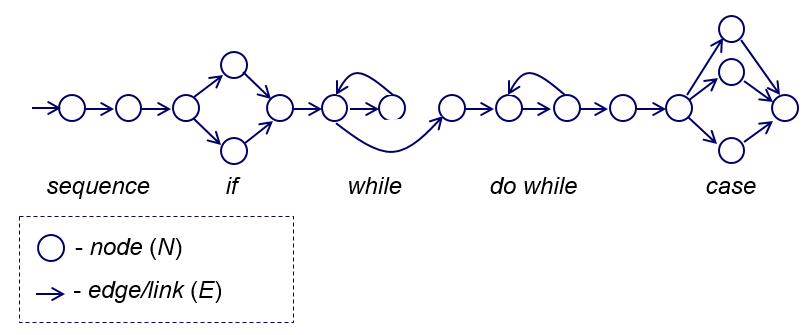
\includegraphics[width=220pt]{gambar/CFG2}
	\caption{Notasi Control Flow Graph (CFG)}
	\label{fig:cfg}
\end{figure}

\textit{Cyclomatic complexity} merupakan suatu sistem pengukuran yang ditemukan oleh \citeauthor{MCCABE} untuk menentukan banyaknya \textit{independent path} dan menunjukan tingkat kompleksitas dari suatu program. \textit{Independent path} adalah jalur yang melintas dalam program yang sekurang-kurangnya terdapat kondisi baru. Perhitungan \textit{Cyclomatic Complexity} dapat dilihat pada persamaan berikut:
\[V(G)=E-N+2\]

Dimana, E menunjukkan jumlah \textit{edges} dan N menunjukkan jumlah \textit{nodes}.

\subsection*{Design}
Pada tahap ini ditentukan bagaimana perangkat lunak akan dibangun. Ilustrasi arsitektur sistem dapat dilihat pada Gambar \ref{fig:struktur}.
\begin{figure}[h!]
	\centering
	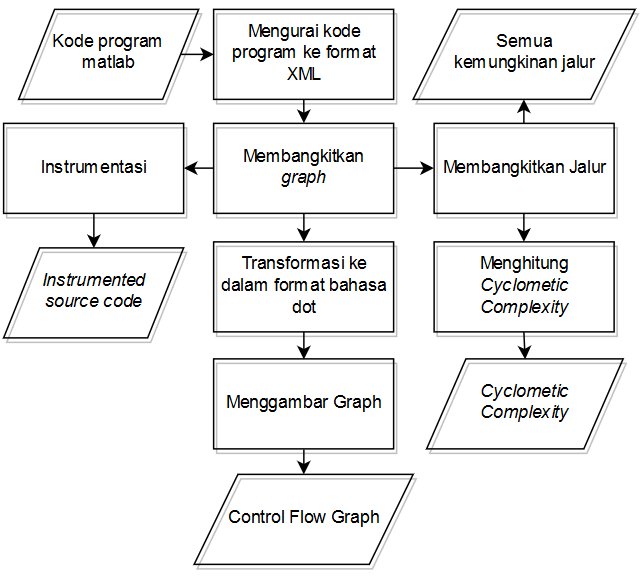
\includegraphics[width=220pt]{gambar/struktur}
	\caption{Arsitektur Sistem}
	\label{fig:struktur}
\end{figure}

\textit{Source code} akan dibaca sebagai inputan, lalu akan dibaca baris perbaris  dengan mengabaikan \textit{whitespace}. Pada tahap awal akan dilakukan akan dilakukan pembangkitan semua jalur yang mungkin dari program dan instrumentasi \textit{source code}. Setelah jalur terbentuk, jalur akan divisualisikan dalam bentuk CFG. 

Instrumentasi merupakan sebuah proses menyisipkan sebuah penanda (tag) di awal atau di akhir setiap blok kode seperti awal setiap fungsi, sebelum atau sesudah kondisi terpenuhi atau tidak. Dalam pengujian \textit{path testing}, penanda ini dapat digunakan untuk memonitor jalur yang dilalui program ketika dijalankan dengan masukan data uji tertentu (\cite{IRH2014})

\subsection*{Implementasi}

Tahapan ini adalah melakukan implementasi dari tahap sebelumnya ke dalam bentuk aplikasi web. Aplikasi ini akan dibangun dengan menggunakan bahasa pemrograman Java dan menggunakan IDE Eclipse. 

Setelah jalur terbentuk, CFG akan divisualisasikan dengan menggunakan library Graphviz. Graphviz merupakan perangkat lunak \textit{open source} untuk visualisasi grafik.

\subsection*{Testing}

Tahapan ini adalah melakukan evaluasi dari tahapan implementasi. Evaluasi dilakukan dengan membandingkan hasil yang dikeluarkan oleh sistem dengan pembangkitan secara manual dari segi waktu eksekusi. 